% ============================================================================
%  Beautified Is Not Forged -- paper v6 (2026-10-17), anonymous submission version. Revision of main_v5.tex with the results of
%  Addenda 38-45 (results/research/retouch_unified_20260929/FINDINGS.md); every change and the source of every new number are in
%  V6_CHANGES.md. Tables: make_tables_v6.py (tab_v6_*, fig_accuse_v6), make_tables_v5.py (tab_v5_*), make_tables_cgd.py.
%  Supplement: supplement_v6.tex. Bibliography: refs_v6.bib.
% ============================================================================
\documentclass[conference]{IEEEtran}
\IEEEoverridecommandlockouts
\usepackage{fontspec}
\setmainfont{texgyretermes}[Extension=.otf,UprightFont=*-regular,BoldFont=*-bold,ItalicFont=*-italic,BoldItalicFont=*-bolditalic]
\usepackage{cite}
\usepackage{amsmath,amssymb,amsfonts}
\usepackage{graphicx}
\usepackage{booktabs}
\usepackage{array}
\usepackage{adjustbox}
\usepackage{xcolor}
\usepackage{url}
\usepackage{capt-of}
\usepackage{xr-hyper}
\usepackage[hidelinks]{hyperref}
\newcommand{\ours}{\textsc{Ours}}
\externaldocument[S-]{supplement_v6}
\graphicspath{{figs/}}
\renewcommand{\dbltopfraction}{0.95}
\renewcommand{\topfraction}{0.95}
\renewcommand{\textfraction}{0.05}
\raggedbottom

\begin{document}

\title{Beautified Is Not Forged: A Two-Sided Measurement of Face-Forgery Detectors under Beautification and Skin Smoothing}

\author{\IEEEauthorblockN{Anonymous submission}}

\IEEEaftertitletext{\vspace{-0.6\baselineskip}\begin{center}
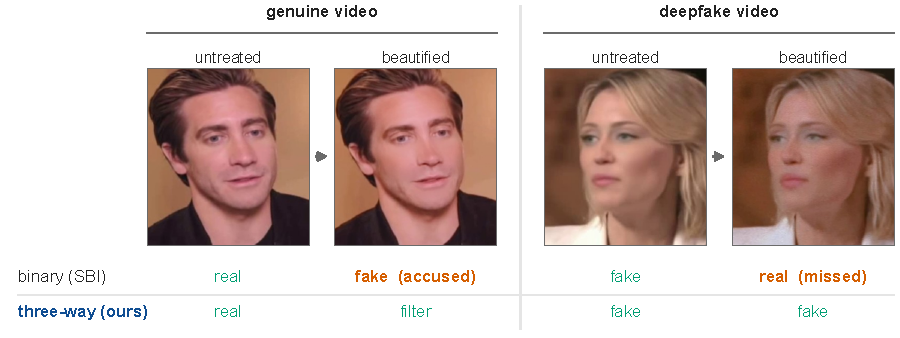
\includegraphics[width=0.84\textwidth]{fig_teaser_v5}
\captionof{figure}{Celeb-DF-B frames of a genuine video and of a deepfake, before and after the same app preset. SBI, at the
threshold that accuses 5\% of untreated genuine frames, accuses the beautified genuine face and lets the beautified deepfake
pass; our full-data three-way model calls the first \emph{filter} and the second \emph{fake} (green: correct, orange: error). The frames were selected where SBI
errs after beautification and our model is correct, so they show the two errors, not their rates. Over the benchmark SBI
accuses 1.8\% of beautified genuine frames and misses 79.8\% of beautified deepfakes; our model accuses 9.5\%, sends 47.4\%
to \emph{filter} and misses 40.7\% (Table~\ref{tab:twosided}).}\label{fig:teaser}
\end{center}\vspace{0.1\baselineskip}}
\maketitle

\begin{abstract}
Many genuine faces reaching a forgery detector were beautified by a camera app, an AR filter or a retouching service. We
measure both errors of seventeen published detectors with one rule: the threshold on the forgery probability accuses 5\% of
each source's untreated genuine faces. All seventeen accuse Instagram AR renders on at least one of two face sets, sixteen on
both. On 2,210 FFHQ originals and their commercial renders, fifteen score strong skin smoothing above the same untouched face in
89--99\% of pairs, and a threshold fixed on FF++ validation still accuses 15--93\% of those faces. Smoothing restricted to the
skin is accused by all seventeen; for the four CLIP-based detectors the forgery logit rises with its strength,
while a radial vignette alone does not move three of them toward forged. In FF++ training the class that receives
beautified views sets the sign of the error: genuine-only smoothing views miss 96--100\% of bilaterally smoothed forgeries, forged-only views
(one seed) raise the accusation of smoothed genuine faces, and views on both classes sit in between. A smoothing view drawn
identically for both classes removes the accusation of whole-crop and commercial smoothing under LoRA tuning of CLIP, not
under Effort's tuning scheme and not for skin-only smoothing (38--99\% false alarms). Our full-data models accuse 0.1--0.5\%
of commercially smoothed faces at the FF++-validation threshold but 75--94\% of AR renders, so our training does not remove
the accusation in general. Evidence maps supervised with exact edit footprints localise held-out part-level forgeries (IoU
0.83).
\end{abstract}

% ----------------------------------------------------------------------------
\section{Introduction}
Face-forgery detectors are used for content moderation, remote identity checks and fact-checking. In these settings a genuine
face called fake accuses a real person, and a forgery called real is let through. Many genuine faces have been beautified:
retouching is common on social media and appears even on identification documents~\cite{bharati2016,rathgeb2019}, skin
smoothing, whitening, eye enlargement and face slimming are default options in camera apps, AR filters and retouching
services, and colour presets ship with every photo-sharing app. Beautification edits the pixels a forgery detector inspects
but does not change who is shown or what the person does. Biometric work has measured its effect on face
recognition~\cite{rathgeb2019} and detected retouching as such~\cite{bharati2016,jain2018}; how it moves a forgery detector in
each direction has been measured for at most six detectors at a time~\cite{libourel2024,saeed2025,concas2025}.

We score seventeen published detectors with one rule that counts both errors: Xception~\cite{xception},
EfficientNet-B4~\cite{efficientnet}, F3Net~\cite{f3net}, SPSL~\cite{spsl}, UCF~\cite{ucf}, RECCE~\cite{recce}, CORE~\cite{core},
SRM~\cite{srm}, SBI~\cite{sbi}, CADDM~\cite{caddm} and LAA-Net~\cite{laanet}, the CLIP-based Effort~\cite{effort}, Forensics
Adapter~\cite{forensicsadapter}, GenD~\cite{gend2026} and DFD-HR~\cite{dfdhr2026}, and two general generated-image detectors,
UnivFD~\cite{univfd} and NPR~\cite{npr}. They are scored on four kinds of beautification: app presets, colour filters, Instagram
AR filters~\cite{openfilter2022}, and a commercial retouching service where each render can be compared with its own original
without a threshold. The largest failure is skin smoothing. The detectors score a smoothed genuine face as more forged than the
same face untouched in nearly every pair, smoothing the skin alone with the background untouched is enough, and for the four
CLIP detectors the forgery logit of a genuine face grows with the smoothing strength. A radial vignette alone does not produce
this shift.

We then ask what training does to these errors, holding architecture, data and recipe fixed and varying only which class
receives beautified views. This is shortcut learning~\cite{geirhos2020} and class-dependent
augmentation~\cite{balestriero2022} in a setting where the sign of the resulting error can be measured. Views on genuine faces
only, the direction of fine-tuning on enhanced genuine samples~\cite{saeed2025}, teach that smoothed means genuine, and a forger
who smooths the forgery is let through; views on forged faces only teach the opposite and accuse smoothed genuine faces. A
smoothing view drawn in the same way for both classes removes the accusation of whole-crop and commercial smoothing for
LoRA-tuned CLIP, at a stated cost in misses on smoothed forgeries; it does not transfer to Effort's tuning scheme or to
skin-only smoothing.

Our contributions are:
\begin{itemize}
\item \textbf{A two-sided measurement with one rule.} Seventeen detectors on four beautification sources, with re-encoding
separated from beautification, a JPEG control for the AR renders, a commercial service read pair by pair, a scripted skin-only
smoothing test, the dose response of the four CLIP detectors, and a threshold fixed on FF++ validation next to the per-source one.
\item \textbf{Which class sees beautification.} Four exposure arms (none, genuine only, both, forged only) showing that the class
receiving the views sets the sign of the error without changing separability, and a pre-registered chain on skin smoothing with
an evasion route, a class-asymmetric form learnt as a label, and a class-symmetric view with its costs and the cases it does not
cover.
\item \textbf{Reference models and a restoration test.} Full-data CLIP models trained with these views, reported with their
weaknesses on two seeds (a binary control trained on the same data detects reenactment better; entire-face synthesis is weak; AR
renders are accused), and evidence maps evaluated by localisation and by restoring the named region.
\end{itemize}
Methods that did not help are summarised in Sec.~\ref{sec:negative}.

% ----------------------------------------------------------------------------
\section{Related Work}
\textbf{Beautification and forgery detection.} Libourel et al.~\cite{libourel2024} released Celeb-DF-B and report video AUC
drops for three detectors under app presets; Saeed et al.~\cite{saeed2025} show that face enhancement lets deepfakes evade six
detectors and fine-tune on enhanced samples; Concas et al.~\cite{concas2025} report both errors for two CNNs under a smoothing
filter. None scores detectors by a common rule or trains against the edit with a class-controlled design. On a million
smartphone photographs, von Stryk and Keuper~\cite{laionmobile2026} find that the false-alarm rate of a generated-image detector
is set by where its threshold was calibrated. OpenFilter~\cite{openfilter2022} renders Instagram AR filters onto FairFace and LFW.
Retouching detection and restoration~\cite{bharati2016,jain2018,wang2019photoshop,
retouchingffhq,frrffusion,mofrr,reface} have no forgery class; Liu et al.~\cite{miea2026} attribute forgery and beautification
tools in a closed set. Perturbation benchmarks for forgery detection~\cite{deeperforensics2020,moire2025} and for
classification~\cite{hendrycks2019} treat edits as corruptions of one class.

\textbf{Shortcuts and attacks.} Shortcut learning~\cite{geirhos2020} and group shifts~\cite{sagawa2020} describe a model that
learns a feature correlated with the label; Balestriero et al.~\cite{balestriero2022} show that augmentation and regularisation
act differently per class. StatAttack~\cite{statattack2023} and AdvShadow~\cite{advshadow2024} optimise natural appearance
changes so that forgeries pass, Fatima et al.~\cite{fatima2025} train on the worst of random counter-forensic transforms, and
semantic adversarial training exists for classification~\cite{hosseini2018,laidlaw2019,gat2023,ava2021}.

\textbf{Generalisable forgery detection.} Face X-ray~\cite{facexray} and SBI~\cite{sbi} synthesise blending artefacts,
UCF~\cite{ucf} separates common from method-specific features, LSDA~\cite{lsda} augments forgery features in latent space for
cross-method generalisation, and Effort, Forensics Adapter, GenD and DFD-HR adapt CLIP ViT-L/14. The alpha-blending
hypothesis~\cite{alphablend2026} holds that frame-based detectors read compositing artefacts, and its authors ensemble a
blending detector with blend-resistant models. DeepfakeBench~\cite{deepfakebench} and DF40~\cite{df40} provide checkpoints and
test sets.

\textbf{Explanations.} Joint detection and segmentation~\cite{nguyen2019multitask,hifinet2023}, attention trained so that
erasing it removes the evidence~\cite{gain}, amortised maskers~\cite{dabkowski2017,phang2020}, DOLOS~\cite{dolos} and
FakeVLM~\cite{fakevlm2025} precede our footprint-supervised maps; our addition is a restoration test against the true footprint.

% ----------------------------------------------------------------------------
\section{Problem and Evaluation Rule}
\label{sec:protocol}
\textbf{Classes.} A face image is \emph{forged} if it shows a person, an expression, a motion or speech that was not captured:
another identity in whole or in part, a reenactment or lip-sync, or a face or a facial feature (eye, nose, mouth) replaced by
new content. It
is \emph{beautified} if its colour, tone, skin texture or the smooth shape of the person's own features were edited after
capture while identity, expression, pose and speech stay those of the capture. The label follows what changed, not the tool: a
retouching service that smooths skin with a neural network beautifies, and a reenactment that keeps the identity forges. The
two attributes are independent, and a beautified forgery is forged. Table~\ref{tab:boundary} lists the cases near the boundary
(the supplement extends it to 17 rows, Table~\ref{S-tab:labels}). Regenerating a part of the same person by inpainting is the
case the wording does not settle: the new part was not captured, so we label it forged, but we have not measured identity or
expression preservation for any edit family, so the boundary is stated, not operationalised.

\begin{table}[t]
\centering
\caption{Cases near the class boundary. ``Scored'': whether a test set of this paper contains the case.}
\label{tab:boundary}
\footnotesize
\setlength{\tabcolsep}{2.5pt}
\begin{tabular}{@{}>{\raggedright\arraybackslash}p{0.47\columnwidth}>{\raggedright\arraybackslash}p{0.2\columnwidth}>{\raggedright\arraybackslash}p{0.27\columnwidth}@{}}
\toprule
Case & Label & Scored \\
\midrule
Colour preset, skin smoothing, whitening, slimming, eye enlargement, AR beauty filter (neural or not) & beautified & presets, filters, AR renders, one service \\
Face swap; reenactment & forged & FF++, Celeb-DF, DFD, DF40 \\
A part from another person & forged & part-level set \\
A part of the same person regenerated by inpainting & forged (boundary) & part-level set \\
Beautified forgery & forged & Celeb-DF-B, smoothed forgeries \\
Entire-face synthesis & forged & DF40, six methods (probe) \\
Attribute editing, lip-sync & forged & not scored (DF40 editing sets not available to us) \\
\bottomrule
\end{tabular}
\end{table}

\textbf{Requirement and rule.} A detector should return a forgery score that does not move when a face is beautified; whether a
face was beautified may be reported to the user as a separate attribute (evaluated in Sec.~\ref{S-sec:native}), and every
detection number reads the forgery score only. Each detector is
scored by its probability of forgery $P(\text{fake})$. On every source the threshold is the one that accuses 5\% of that
source's untreated genuine frames. It is fitted per source, which no deployed detector can do, so we also report one
deployable threshold per detector, the 95th percentile of its scores on the 530 genuine FF++ c23 validation frames (133 videos),
and on the retouching service statistics that need no threshold. Under
beautification we report the false-alarm rate FA (genuine faces called fake) and the miss rate MISS (forgeries not called
fake). A forgery that a three-way model sends to its beautified class is a miss. Every AUC is labelled frame or video level;
video scores are means of frame scores. Intervals are 95\% percentile bootstraps that resample videos (Celeb-DF-B, the filter
sources, DF40), originals (the service) or pairs (AR renders), with the threshold re-estimated in every draw: 1,000 draws, 500
for the filter sources. We repeated every interval on the video sources with identities as the resampling unit
(Sec.~\ref{S-sec:identity}); where this changes a reading the text says so. Differences between models use identical
draws. We do not correct for multiple comparisons except where stated.

\textbf{Sources.} \emph{Celeb-DF-B}~\cite{libourel2024}: 232 Celeb-DF-v2 videos per condition (as recorded, re-encoded,
beautified by one of four app presets; genuine and synthesised), 32 frames each; 231 have a detected face in the untreated
and 230 in the beautified genuine condition. The treated videos are re-framed to portrait with tinted bars, and our face
detector missed 57\% of their faces; after reading that result we trimmed uniform bars from all six conditions before
detection. This fix is post hoc, and face size and resampling still differ between untreated and treated frames, which the
re-encoded control does not reproduce. We report re-encoding alone and its difference from the preset on both errors:
$\Delta$MISS$_\text{beauty}$ and $\Delta$FA$_\text{beauty}$ are the rise under the preset minus the rise under re-encoding,
and AUC$_c{-}$AUC$_b$ is the AUC lost beyond re-encoding. \emph{Celeb-DF-v2 filters}: 516 test videos~\cite{celebdf}, each
frame also under one of eleven colour filters~\cite{pilgram} never used in training; this set was used to diagnose the filter
effect and is a development source. \emph{DFD filters}: 332 DFD videos~\cite{dfd} under one of sixteen filters from a second
library, built after every method decision. \emph{AR filters}~\cite{openfilter2022}: FairBeauty, 2,927 FairFace photographs and
their Instagram AR renders (eight distinct filters), and B-LFW, 3,000 of its 11,891 LFW pairs (2,016 identities). The AR engine
re-renders the face through its own capture path, so we also score FairBeauty with both sides re-compressed (JPEG q90); the AR
numbers are an upper bound on the effect of the beautification itself. \emph{Commercial retouching}: 2,210 FFHQ originals and
their renders by Alibaba from RetouchingFFHQ~\cite{retouchingffhq} (four operations, three levels). No model was trained on
this service, but more than 60 of our checkpoints and all 17 published detectors have been scored on it, the strongest
smoothing level (Smoothing-90) was singled out after reading it, and the pre-declared bars of Sec.~\ref{sec:chain} are defined
on it; it is an analysis set, not a clean test. Its originals share no image with the 7,831 FFHQ training originals (a
disjoint index range; FFHQ has no identity labels). \emph{Scripted smoothing}: 4,016 Celeb-DF-v2 test frames (1,348 genuine,
513 videos) with a whole-crop bilateral filter at three strengths, a median filter, a Gaussian blend, and a bilateral filter
inside the landmark face hull at two strengths (\emph{face-local}, background untouched), applied to both classes.
\emph{Untreated detection}: Celeb-DF-v2, DFD and the held-out methods of DF40~\cite{df40}.

\begin{table}[t]
\centering
\caption{Models and arms. All use CLIP ViT-L/14 with rank-16 LoRA (or Effort's SVD-residual tuning where noted) and the
training pipeline of Sec.~\ref{sec:method}. ``Views'': which class receives beautified training views.}
\label{tab:notation}
\footnotesize
\setlength{\tabcolsep}{2.5pt}
\begin{tabular}{@{}>{\raggedright\arraybackslash}p{0.27\columnwidth}>{\raggedright\arraybackslash}p{0.56\columnwidth}c@{}}
\toprule
Name & Data, views, head & seeds \\
\midrule
P0, P1, P2 & FF++ only, forged head; views on no class, genuine only, both & 3 \\
P3 & as P0, views on forged faces only & 1 \\
P1-smooth & P1 with smoothing as the only view & 3 \\
P2-smooth, P2-nosmooth & P2 with smoothing only, with smoothing removed & 2 \\
P2-sym & smoothing as the only view, same form on both classes & 2 \\
Effort scheme & P0 and P2 (2 seeds), P2-sym (1 seed), SVD-residual tuning & 1--2 \\
\ours{} & full data$^\dagger$, P2 views, three-way head & 2 \\
\ours{} variant & \ours{} with the class-symmetric smoothing view & 2 \\
binary control & \ours{} data and views, forged head only & 2 \\
\bottomrule
\multicolumn{3}{@{}p{0.97\columnwidth}@{}}{\scriptsize $^\dagger$FF++ plus 7,831 FFHQ originals, their renders by two retouching services (Tencent, Megvii) and the single-operation components of those renders, and 61,510 part-level forgeries. The published CLIP detectors were trained on FF++ alone.}\\
\end{tabular}
\end{table}

% ----------------------------------------------------------------------------
\section{Method}
\label{sec:method}
Every edited training image has a pixel-aligned original $x_0$, so the footprint of the edit is exact,
$M(x)=\mathrm{dilate}_\rho(\mathbf{1}[\|x-x_0\|_\infty>\tau])$ with $\tau=6$ on 8-bit intensities.

\textbf{FF++ triplets.} FF++ c23~\cite{ffpp}, official 720/140/140 video split. For each genuine training frame $x_0$ a step
draws a genuine item, a beautified item (one of four landmark and skin operations at a random strength, one of 14 colour
filters~\cite{pilgram}, or a random colour grading) and a forged item (a self-blend of $x_0$~\cite{sbi}, an observed FF++
forgery, or a part-level forgery), and the forged item is beautified with probability 0.5. Forged items without landmarks
receive skin smoothing as a whole-crop filter, not as the face-local operation; Sec.~\ref{sec:chain} shows what this asymmetry
teaches. The same random blur or downscale is applied to all three items. The FF++-only arms use nothing else.

\textbf{Commercial renders and part-level forgeries.} The full-data models add 7,831 FFHQ photographs~\cite{ffhq} and their
renders by Tencent and Megvii~\cite{retouchingffhq}, sister services of the test service with the same four operations. Each
render is split by dense optical flow~\cite{dis} and a photometric residual into eye and contour warps and low- and
high-frequency photometric components in the original's geometry (supplement, Alg.~\ref{S-alg:decomp}); 50,112 of 73,952
components lie above the noise floor. A render's photometric residual is also added to a self-blend of the same original.
61,510 part-level forgeries on FF++ frames transplant the eyes, nose or mouth of another identity or regenerate the part with
Stable Diffusion inpainting, with pixels outside the feathered mask copied from $x_0$; the held-out set uses test frames and
test donors.

\textbf{Model.} A frozen CLIP ViT-L/14~\cite{clip} with rank-16 LoRA~\cite{lora} on every attention projection (3.2\,M of
306\,M parameters trained). Two linear heads on the pooled feature give the forged logit $z_f$ and the beautified logit $z_b$;
$P(\text{fake})=\sigma(z_f)$ and $P(\text{filter})=(1-\sigma_f)\sigma_b$, so the forgery score does not depend on $z_b$. An
operation-presence head and a $1\times1$ convolution on the spatial tokens (the evidence map $\hat m$, $16\times16$) are
trained against the operation labels and $M$ with BCE and Dice; the classifier does not read $\hat m$. Training: 224\,px,
AdamW at $10^{-4}$, 8 epochs, 16 genuine bases per batch. Checkpoints are chosen on validation data only (FF++ validation
macro-F1; for full-data models its mean with balanced accuracy on held-out originals and renders of the training services).

% ----------------------------------------------------------------------------
\section{Results}
\label{sec:results}
\begin{table*}[t]
\centering
\caption{Both errors under one rule ($P(\text{fake})$, threshold at 5\% FPR on each source's untreated genuine frames).
Celeb-DF-B: AUC untreated, re-encoded (AUC$_c$) and beautified (AUC$_b$), AUC lost beyond re-encoding, rise in misses and in
false alarms under the preset minus the rise under re-encoding, and FA$_b$, the false-alarm rate on beautified genuine frames.
DFD: sixteen held-out filters on the full frame. Percentage points. Intervals, the Celeb-DF-v2 filter source and video-level
AUC in the supplement (Tables~\ref{S-tab:twosidedfull} and~\ref{S-tab:cdfbextra}). $^\ddagger$General generated-image detectors,
not trained on faces. $^\dagger$Trained on more data than the published detectors (Table~\ref{tab:notation}).}
\label{tab:twosided}
\scriptsize
\setlength{\tabcolsep}{3pt}
\begin{adjustbox}{max width=\textwidth}\begin{tabular}{@{}ll ccccccc cccc@{}}
\toprule
 & & \multicolumn{7}{c}{Celeb-DF-B, app presets (frame level)} & \multicolumn{4}{c}{DFD + 16 held-out filters (frame level)} \\
\cmidrule(lr){3-9}\cmidrule(lr){10-13}
Detector & train & AUC & AUC$_c$ & AUC$_b$ & AUC$_c{-}$AUC$_b$ & $\Delta$MISS$_\text{beauty}$ & FA$_b$ & $\Delta$FA$_\text{beauty}$ & AUC & AUC$_f$ & $\Delta$MISS & $\Delta$FA \\
\midrule
Xception~\cite{xception} & FF++ c23 & 0.811 & 0.795 & 0.737 & 0.058 & +10.9 & 5.7 & -1.7 & 0.854 & 0.834 & +2.0 & +2.0 \\
EfficientNet-B4~\cite{efficientnet} & FF++ c23 & 0.811 & 0.798 & 0.762 & 0.035 & +3.4 & 7.8 & +1.7 & 0.810 & 0.781 & +6.3 & -0.5 \\
F3Net~\cite{f3net} & FF++ c23 & 0.798 & 0.782 & 0.731 & 0.051 & +10.9 & 5.4 & -1.9 & 0.781 & 0.774 & -8.5 & +3.6 \\
SPSL~\cite{spsl} & FF++ c23 & 0.781 & 0.769 & 0.727 & 0.042 & +12.4 & 3.4 & -2.4 & 0.829 & 0.837 & +4.7 & -1.8 \\
UCF~\cite{ucf} & FF++ c23 & 0.841 & 0.829 & 0.777 & 0.053 & +11.3 & 5.7 & +0.2 & 0.822 & 0.804 & +5.0 & +0.3 \\
RECCE~\cite{recce} & FF++ c23 & 0.785 & 0.765 & 0.723 & 0.042 & +13.8 & 4.1 & -3.6 & 0.833 & 0.808 & +7.3 & -0.2 \\
CORE~\cite{core} & FF++ c23 & 0.821 & 0.808 & 0.752 & 0.057 & +13.5 & 4.0 & -2.2 & 0.827 & 0.821 & -5.4 & +1.6 \\
SRM~\cite{srm} & FF++ c23 & 0.789 & 0.769 & 0.733 & 0.035 & +15.3 & 2.8 & -3.4 & 0.830 & 0.822 & +5.8 & +0.2 \\
SBI~\cite{sbi} & FF++ c23 & 0.875 & 0.861 & 0.752 & 0.109 & +21.8 & 1.8 & -0.6 & 0.829 & 0.810 & +4.5 & +0.4 \\
UnivFD$^\ddagger$~\cite{univfd} & ProGAN$^\ddagger$ & 0.653 & 0.637 & 0.624 & 0.013 & -7.2 & 7.6 & +4.5 & 0.840 & 0.801 & -10.2 & +11.6 \\
NPR$^\ddagger$~\cite{npr} & ProGAN$^\ddagger$ & 0.503 & 0.503 & 0.498 & 0.006 & -0.7 & 3.4 & +0.9 & 0.473 & 0.516 & -13.7 & +9.4 \\
Effort~\cite{effort} & FF++ c23 & 0.909 & 0.882 & 0.807 & 0.075 & +11.0 & 5.4 & +2.1 & 0.939 & 0.905 & +15.1 & -2.3 \\
Forensics Adapter~\cite{forensicsadapter} & FF++ c23 & 0.909 & 0.894 & 0.828 & 0.066 & +15.2 & 7.9 & +0.1 & 0.940 & 0.924 & +8.0 & -0.6 \\
GenD~\cite{gend2026} & FF++ c23 & 0.924 & 0.898 & 0.807 & 0.091 & +12.0 & 9.9 & +3.6 & 0.934 & 0.925 & +3.1 & +1.2 \\
DFD-HR~\cite{dfdhr2026} & FF++ c23 & 0.938 & 0.915 & 0.838 & 0.077 & +3.6 & 14.6 & +9.8 & 0.943 & 0.928 & +9.1 & -2.0 \\
CADDM~\cite{caddm} & FF++ raw & 0.886 & 0.850 & 0.762 & 0.088 & -2.9 & 13.8 & +9.9 & 0.845 & 0.818 & +3.8 & +0.8 \\
LAA-Net~\cite{laanet} & FF++ raw & 0.889 & 0.870 & 0.698 & 0.172 & +14.7 & 6.0 & +3.3 & 0.810 & 0.783 & +6.2 & +0.0 \\
\midrule
P0 & FF++ & 0.927 & 0.901 & 0.860 & 0.041 & +17.0 & 5.1 & -1.6 & 0.943 & 0.924 & +9.3 & -0.2 \\
P2-sym & FF++ & 0.920 & 0.900 & 0.866 & 0.034 & +14.2 & 5.5 & -1.2 & 0.936 & 0.921 & +7.3 & -0.4 \\
\ours{}$^\dagger$ & FF++, FFHQ & 0.938 & 0.918 & 0.866 & 0.052 & +6.7 & 9.5 & +4.9 & 0.942 & 0.931 & +8.9 & -1.0 \\
\quad second seed$^\dagger$ & FF++, FFHQ & 0.941 & 0.926 & 0.883 & 0.043 & +8.3 & 6.7 & +2.7 & 0.945 & 0.931 & +4.4 & +0.3 \\
\quad \ours{} variant$^\dagger$ & FF++, FFHQ & 0.941 & 0.925 & 0.868 & 0.057 & +10.0 & 9.2 & +4.9 & 0.947 & 0.934 & +8.5 & -0.9 \\
binary control$^\dagger$ & FF++, FFHQ & 0.949 & 0.934 & 0.896 & 0.038 & +7.0 & 7.4 & +2.3 & 0.961 & 0.952 & +4.2 & +0.2 \\
\bottomrule
\end{tabular}
\end{adjustbox}
\end{table*}

\begin{table}[t]
\centering
\caption{Commercial skin smoothing (Smoothing-90): 2,210 FFHQ originals and their renders. Share of renders scored above their
own original (50 means no shift), medians of $P(\text{fake})$, median paired shift of the forgery logit with a bootstrap
interval over originals, share of renders above the threshold that accuses 5\% of the originals, and share above the
threshold fixed on FF++ validation. NPR scores everything at 1.0.}
\label{tab:retouch}
\scriptsize
\setlength{\tabcolsep}{2pt}
\begin{adjustbox}{max width=\columnwidth}\begin{tabular}{@{}l ccccc@{}}
\toprule
Detector & above own orig.\ (\%) & median $P(\text{fake})$ & median $\Delta$logit [95\% CI] & accused (\%) & FF++-val.\ thr.\ (\%) \\
\midrule
Xception~\cite{xception} & 95.2 & 0.29 $\rightarrow$ 0.94 & +3.32 [+3.17, +3.45] & 51.6 & 65.0 \\
EfficientNet-B4~\cite{efficientnet} & 93.7 & 0.32 $\rightarrow$ 0.96 & +3.48 [+3.33, +3.57] & 36.3 & 63.8 \\
F3Net~\cite{f3net} & 97.8 & 0.13 $\rightarrow$ 0.97 & +4.92 [+4.74, +5.08] & 50.6 & 69.0 \\
SPSL~\cite{spsl} & 97.3 & 0.46 $\rightarrow$ 0.96 & +3.05 [+2.95, +3.12] & 51.2 & 56.3 \\
UCF~\cite{ucf} & 95.4 & 0.03 $\rightarrow$ 0.98 & +5.47 [+5.20, +5.73] & 41.4 & 48.4 \\
RECCE~\cite{recce} & 96.5 & 0.12 $\rightarrow$ 0.94 & +3.82 [+3.70, +3.96] & 36.8 & 60.0 \\
CORE~\cite{core} & 96.6 & 0.25 $\rightarrow$ 0.95 & +3.90 [+3.74, +4.03] & 54.8 & 66.7 \\
SRM~\cite{srm} & 99.3 & 0.46 $\rightarrow$ 0.67 & +0.68 [+0.65, +0.71] & 62.8 & 62.0 \\
SBI~\cite{sbi} & 96.2 & 0.21 $\rightarrow$ 0.99 & +4.88 [+4.72, +5.04] & 37.3 & 93.3 \\
UnivFD$^\ddagger$~\cite{univfd} & 90.4 & 0.01 $\rightarrow$ 0.02 & +1.22 [+1.17, +1.28] & 16.6 & 15.2 \\
NPR$^\ddagger$~\cite{npr} & n/a & n/a & n/a & n/a & n/a \\
Effort~\cite{effort} & 95.6 & 0.32 $\rightarrow$ 0.59 & +0.96 [+0.90, +1.02] & 43.2 & 31.1 \\
Forensics Adapter~\cite{forensicsadapter} & 93.3 & 0.06 $\rightarrow$ 0.35 & +1.72 [+1.59, +1.87] & 39.7 & 32.5 \\
GenD~\cite{gend2026} & 98.5 & 0.23 $\rightarrow$ 0.92 & +3.27 [+3.19, +3.35] & 68.7 & 67.4 \\
DFD-HR~\cite{dfdhr2026} & 99.0 & 0.21 $\rightarrow$ 0.71 & +2.06 [+1.93, +2.15] & 64.9 & 56.2 \\
CADDM~\cite{caddm} & 60.9 & 0.54 $\rightarrow$ 0.74 & +0.67 [+0.53, +0.81] & 6.3 & 42.3 \\
LAA-Net~\cite{laanet} & 89.2 & 0.23 $\rightarrow$ 0.97 & +3.60 [+3.36, +3.79] & 17.2 & 81.0 \\
\midrule
P0 & 98.5 & 0.05 $\rightarrow$ 0.97 & +5.17 [+5.05, +5.38] & 54.2 & -- \\
P2-sym & 53.7 & 0.02 $\rightarrow$ 0.02 & +0.09 [+0.03, +0.12] & 5.9 & -- \\
\ours{}$^\dagger$ & 32.5 & 0.00 $\rightarrow$ 0.00 & -1.20 [-1.28, -1.12] & 8.6 & 0.5 \\
\quad \ours{} variant$^\dagger$ & 30.0 & 0.00 $\rightarrow$ 0.00 & -1.09 [-1.19, -1.00] & 8.1 & 0.1 \\
binary control$^\dagger$ & 70.5 & 0.00 $\rightarrow$ 0.00 & +0.41 [+0.38, +0.44] & 9.1 & 0.2 \\
\bottomrule
\end{tabular}
\end{adjustbox}
\end{table}

\begin{figure}[t]
\centering
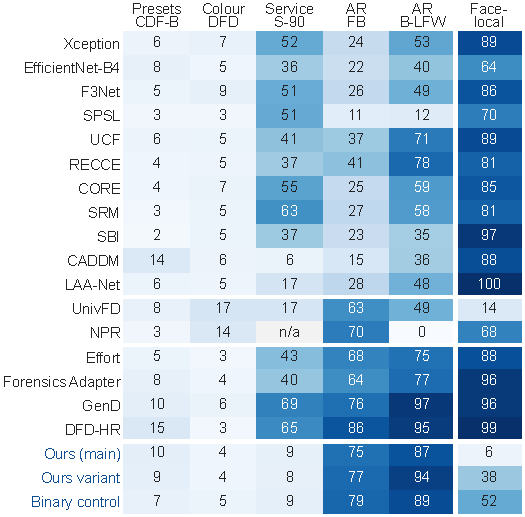
\includegraphics[width=\columnwidth]{fig_accuse_v6}
\caption{Accused share of beautified genuine faces (\%) at the threshold that accuses 5\% of each source's untreated genuine
faces: Celeb-DF-B presets (FA$_b$), DFD under sixteen colour filters, commercial Smoothing-90, Instagram AR renders of
FairBeauty (FB) and B-LFW, and the scripted face-local smoothing of Celeb-DF-v2 genuine frames (strength 0.06). Rows: eleven
face-forgery CNNs, two general detectors, four CLIP detectors, and our full-data models (first seed). NPR is saturated on the
service.}
\label{fig:accuse}
\end{figure}

\subsection{Both errors under one rule}
\label{sec:measure}
\textbf{Commercial retouching.} Table~\ref{tab:retouch} reads the Smoothing-90 renders against their own originals. Fifteen of
the seventeen detectors score the render above its original in 89--99\% of pairs, and the median $P(\text{fake})$ moves from
0.21 to 0.99 for SBI and from 0.23 to 0.92 for GenD: a heavily smoothed genuine face is scored like a forgery whatever the
threshold. The exceptions are NPR, saturated, and CADDM (60.9\%). At the threshold that accuses 5\% of the originals thirteen
detectors accuse 36.3--68.7\% of the renders. Whitening, face slimming and eye enlarging at their strongest level stay at
3.7--8.1\% for thirteen of the sixteen detectors other than NPR (Table~\ref{S-tab:v4perop}); these operations go through the same
service, encoder and resolution as the smoothing, so the retouching result is a smoothing result. A sign test rejects ``no
shift'' for every published detector other than NPR ($p<10^{-10}$), with median paired logit shifts of $+0.7$ to $+5.5$. Our
full-data three-way models move the other way: \ours{} scores the render \emph{below} its original in 67.5\% of pairs (median
$-1.20$ [$-1.28$, $-1.12$]; second seed $-0.53$). Only the FF++-only symmetric arm P2-sym stays close to no shift ($+0.09$
[$+0.03$, $+0.12$] and $+0.03$ [$0.00$, $+0.09$]). Our full-data models were trained on renders of the two sister services
(marked $^\dagger$), which the published detectors were not.

\textbf{A deployable threshold.} With the threshold fixed on FF++ validation (last column), the published detectors accuse
15.2\% (UnivFD) to 93.3\% (SBI) of the Smoothing-90 renders, and CADDM and LAA-Net, which accuse 6.3 and 17.2\% under the
per-source rule, accuse 42.3 and 81.0\%: their scores drift on untreated stills, and SBI, CADDM and LAA-Net already call 45.3,
32.9 and 30.9\% of the untouched FFHQ originals fake. Our models accuse 0.1--0.5\% (both seeds); they were trained on FFHQ
stills and sister-service renders, so this is partly ``trained on stills of this kind''. The detector ranking by accused share
is not stable under the change of rule (Spearman between the two rules 0.29, $p=0.25$, on the service; 0.37, $p=0.15$, on
FairBeauty), so the threshold-free columns are the ones to read first (Table~\ref{S-tab:deploy}).

\textbf{Instagram AR filters.} Under the per-source rule all seventeen detectors accuse FairBeauty renders above the 5\% floor
(lower interval bound above 5\%; 10.7--85.9\%) and sixteen accuse B-LFW renders (12.0--96.6\%); NPR's scores saturate on the
112\,px B-LFW renders. Every published detector ranks the FairBeauty render above its own original in 68.9--98.8\% of pairs,
and all but NPR rank the B-LFW render above it in 80.7--99.9\% (Fig.~\ref{fig:accuse}, Table~\ref{S-tab:ar}). With both sides of FairBeauty re-compressed, every detector except NPR
keeps 0.64--1.05 of its accused share, so re-compression does not carry the effect, although the AR capture path remains
confounded with the beautification. Which detectors accuse most depends on the source (Spearman of the FairBeauty and service
shares over the seventeen 0.15, $p=0.58$); that every detector accuses does not. Our models are not exempt: \ours{} accuses
75.1\% of FairBeauty and 86.7\% of B-LFW renders, more than Effort and Forensics Adapter (paired $+7.4$ [$+4.4$, $+11.5$] and
$+11.2$ [$+8.2$, $+14.2$] on FairBeauty), on par with GenD and below DFD-HR; the variant and the binary control accuse
75.6--82.1\% and 89.0--94.3\% on two seeds each. At the FF++-validation threshold \ours{} also calls 19.1\% of the untouched
FairFace originals fake. Our training removes the accusation on the vendor family it saw, not on AR filters.

\textbf{Skin-only smoothing.} A bilateral filter inside the face hull, with the background untouched, is accused by all seventeen
detectors (Fig.~\ref{fig:accuse}, Table~\ref{S-tab:smooth38}): the four CLIP detectors call 87.8--99.3\% of genuine frames forged at
the milder strength and 99.9--100\% at the stronger one, the eleven face-forgery CNNs 64.3--100\% and 91.8--100\%, UnivFD 13.9
and 55.2\%, NPR 68.0 and 77.7\%. At matched visible strength skin-only smoothing is accused more often than whole-crop smoothing.
The smoothing of the skin is enough to be called forged.

\textbf{App presets.} On Celeb-DF-B every detector that detects the untreated forgeries loses frame AUC beyond what
re-encoding costs (Table~\ref{tab:twosided}): SBI 0.861 to 0.752 against the re-encoded frames, CADDM 0.850 to 0.762, LAA-Net
0.870 to 0.698, and 0.066--0.091 for the four CLIP detectors. At video level CADDM goes from 0.965 to 0.832 (0.933 re-encoded),
against 0.91 to 0.76 reported by Libourel et al.~\cite{libourel2024}. Here the errors fall mostly on the miss side: beyond
re-encoding, the presets raise the miss rate by 21.8 (SBI), 11.0 (Effort), 15.2 (Forensics Adapter), 12.0 (GenD) and 14.7 points
(LAA-Net), and raise false alarms by 9.8 (DFD-HR), 9.9 (CADDM) and 3.6 points (GenD). CADDM's misses do not rise ($-2.9$; under
identity resampling its interval contains zero) because the presets raise its scores for genuine frames too. Under the DFD filters
Effort's miss rate rises by 15.1 points and Forensics Adapter's by 8.0.

\subsection{Dose response}
\label{sec:mechanism}
On the 1,348 genuine Celeb-DF-v2 frames we varied the strength of three edits and read the forgery logit of the four released CLIP
detectors (Table~\ref{S-tab:dose}). Under face-local smoothing the logit rises in at least 97.9\% of frames at every level for all
four and the median shift grows with strength; the weakest level (0.03) already moves the median logit by $+2.40$ (Effort) to $+4.58$ (Forensics Adapter),
1.0--1.9 times the gap between the mean forged and the mean genuine logit of the detector, and the strongest by 1.9--3.0 gaps.
Whole-crop bilateral smoothing gives the same picture at smaller shifts (1.0--1.7 gaps at the strongest strength). A radial
vignette alone does not: Effort, Forensics Adapter and GenD move the other way ($-0.2$ to $-0.4$ at strength 0.8), and DFD-HR
passes the monotonicity rule with a shift of 3\% of its gap. For the published CLIP detectors smoothing is the operative edit, and
a genuine face is pushed past the forged mean. The vignette result corrects the earlier reading of a probe of one FF++-only model of
ours, in which the two held-out filters with a radial luminance overlay moved the forgery logit of genuine frames by $+7.8$ and
$+5.6$ against $+0.1$ to $+2.4$ for pure colour looks (Sec.~\ref{S-sec:probe}): that effect belongs to that model and does not
appear in the released detectors when the vignette is isolated; erasing that model's beautification subspace does not lower
its false alarms (Table~\ref{S-tab:erasure}).

\subsection{Which class receives beautified views}
\label{sec:exposure}
With architecture, data and recipe fixed, P0--P3 differ only in which class receives beautified views
(Table~\ref{tab:notation}). On Celeb-DF-B the beautification-specific miss rise is 17.0, 14.2 and 10.8 points for P0 (three
seeds), 21.5, 21.8 and 20.4 for P1 and 9.8, 10.3 and 12.8 for P2 (Table~\ref{S-tab:exposure}). P1 exceeds P0 by 4.5--9.5 points
in every seed and P2 by 7.5--11.7; all three P1$-$P0 contrasts remain significant after a Holm correction over the nine exposure
contrasts (adjusted $p\le0.01$). P2 against P0 is $-7.2$, $-4.0$ and $+2.0$ points: of changing sign and within the seed spread of
P0. On the two filter sources P2 lowers the miss rise by 5--10 points in 9 of 10 seed-by-source cells and raises the false-alarm
rise by 2--5 points, while the frame AUC under the filters does not change.

The forged-only arm P3 (one seed, pre-declared reading) completes the design and mirrors P1 on every source
(Table~\ref{tab:tradeoff}, Table~\ref{S-tab:p3}). It accuses 63.8\% [59.0, 67.8] of the Smoothing-90 renders ($+9.6$ [$+6.0$, $+13.4$]
over P0), 99.5 and 100\% of mid and strong whole-crop-smoothed genuine frames (P0: 16.8 and 39.6\%) and 98.1--100\% of
skin-only-smoothed ones. Smoothed, filtered or beautified forgeries are caught more often than untreated ones (miss change
$-25.1$ points under the Celeb-DF-v2 filters and $-6.6$ under the DFD filters), and genuine faces pay for it (47.2\% of filtered
Celeb-DF-v2 genuine frames and 24.6\% of beautified Celeb-DF-B genuine frames accused, against 18.8 and 5.1\% for P0). The sign
rule holds: genuine-only views lower the accusation and open evasion, forged-only views raise the accusation and close evasion,
and views on both classes sit in between. Exposure moves errors between misses and false alarms; it does not make the classes more
separable (P3 untreated Celeb-DF-v2 video AUC 0.943 against 0.938 for P0). Under Effort's tuning scheme P2 also lowers the miss
rise against P0 ($-4.6$ and $-5.2$ points, two seeds); P1 and P3 were not trained under that scheme. The no-exposure CLIP model
already keeps more frame AUC under the presets (0.860--0.883) than Effort's released checkpoint (0.807), so most of the margin of
our models over the CLIP baselines comes from the base recipe, not from exposure.

\begin{table*}[t]
\centering
\caption{What each training recipe buys and costs, per seed (1 / 2 / 3 where trained; ``--'' not scored); names as in
Table~\ref{tab:notation}. Commercial Smoothing-90 as in Table~\ref{tab:retouch}. Smoothed Celeb-DF-v2: change of the miss rate on
forgeries under the strong whole-crop bilateral filter at the threshold of 5\% FPR on untreated genuine frames (a negative value
comes from accusing every smoothed frame, genuine ones included), and frame AUC with both classes smoothed. Untreated Celeb-DF-v2
video AUC; Celeb-DF-B frame AUC under the presets; DF40 reenactment (FR) in the FF++ domain, video AUC, mean over twelve methods.
DFD, $\Delta$MISS$_\text{beauty}$, the Celeb-DF domain, every smoothing form and intervals in
Tables~\ref{S-tab:tradeofffull}, \ref{S-tab:v4evasion}, \ref{S-tab:smooth38} and~\ref{S-tab:v4df40full}.}
\label{tab:tradeoff}
\scriptsize
\setlength{\tabcolsep}{2.5pt}
\begin{adjustbox}{max width=\textwidth}\begin{tabular}{@{}l cc cc c c c@{}}
\toprule
 & \multicolumn{2}{c}{commercial Smoothing-90} & \multicolumn{2}{c}{smoothed Celeb-DF-v2} & Celeb-DF-v2 & Celeb-DF-B & DF40 FR \\
\cmidrule(lr){2-3}\cmidrule(lr){4-5}
Arm & accused (\%) & above own orig.\ (\%) & miss rise & frame AUC & video AUC & frame AUC$_b$ & video AUC \\
\midrule
P0 & 54.2 / 56.1 / 43.5 & 98.5 / 99.0 / 97.0 & -16.0 / -11.8 / +4.3 & 0.747 / 0.736 / 0.736 & 0.938 / 0.938 / 0.940 & 0.860 / 0.883 / 0.883 & 0.906 / 0.877 / 0.873 \\
P1 & 3.7 / 7.1 / 4.6 & 43.5 / 67.5 / 64.3 & +51.2 / -- / -- & 0.587 / -- / -- & 0.900 / 0.910 / 0.923 & 0.844 / 0.851 / 0.864 & 0.807 / -- / -- \\
P2 & 11.7 / 7.1 / 6.9 & 84.1 / 72.4 / 75.5 & -26.5 / -13.3 / -- & 0.740 / 0.746 / -- & 0.917 / 0.920 / 0.935 & 0.879 / 0.893 / 0.877 & 0.809 / 0.785 / -- \\
P3 & 63.8 & 99.2 & -38.5 & 0.743 & 0.943 & 0.857 & 0.870 \\
P2-nosmooth & 55.3 / 67.1 & 98.6 / 99.4 & -28.9 / -33.1 & 0.732 / 0.695 & 0.913 / 0.924 & 0.879 / 0.873 & 0.858 / -- \\
P2-smooth & 2.3 / 5.3 & 27.3 / 51.7 & -48.2 / -44.6 & 0.785 / 0.734 & 0.904 / 0.926 & 0.865 / 0.870 & 0.779 / 0.833 \\
P1-smooth & 0.7 / 1.0 / 0.9 & 2.6 / 6.5 / 5.4 & +56.4 / +60.0 / +62.9 & 0.643 / 0.579 / 0.596 & 0.922 / 0.929 / 0.939 & 0.887 / 0.896 / 0.893 & 0.871 / 0.869 / 0.900 \\
P2-sym & 5.9 / 6.1 & 53.7 / 51.8 & +14.6 / +17.5 & 0.767 / 0.796 & 0.919 / 0.934 & 0.866 / 0.888 & 0.871 / 0.796 \\
Effort scheme, P0 & 56.9 / 63.2 & 99.1 / 99.1 & -32.2 / -- & 0.719 / -- & 0.944 / 0.954 & 0.882 / 0.886 & -- / -- \\
Effort scheme, P2-sym & 14.5 & 88.4 & +24.9 & 0.757 & 0.935 & 0.890 & 0.822 \\
released Effort fine-tuned, no views & 55.3 & 98.5 & -39.9 & 0.754 & 0.926 & 0.805 & -- \\
released Effort fine-tuned, P2-sym view & 39.9 & 96.6 & -19.0 & 0.740 & 0.921 & 0.791 & 0.805 \\
\ours{} & 8.6 / 12.5 & 32.5 / 41.3 & -44.3 / -46.7 & 0.688 / 0.711 & 0.947 / 0.946 & 0.866 / 0.883 & 0.718 / 0.780 \\
\ours{} variant & 8.1 / 17.8 & 30.0 / 46.2 & +34.1 / +11.6 & 0.796 / 0.784 & 0.954 / 0.953 & 0.868 / 0.888 & 0.738 / 0.718 \\
binary control & 9.1 / 6.5 & 70.5 / 68.2 & -15.0 / +2.2 & 0.754 / 0.810 & 0.956 / 0.963 & 0.896 / 0.904 & 0.842 / 0.856 \\
\bottomrule
\end{tabular}
\end{adjustbox}
\end{table*}

\subsection{Skin smoothing: a chain of pre-registered arms}
\label{sec:chain}
We traced the smoothing result through FF++-only arms, each with bars written before training (Table~\ref{tab:tradeoff},
Sec.~\ref{S-sec:chain}); no retouching-service image is used. The scripted smoothing range was set to cover the two sister
services while the test service's measurements were on disk, and the first analysis on the service (P0, P1, P2) was post hoc.

\textbf{No exposure reproduces the published detectors.} P0 accuses 54.2, 56.1 and 43.5\% of the Smoothing-90 renders and
scores them above their original in 97--99\% of pairs, although it trains with label-symmetric blur, rescaling and JPEG.
General beautified views lower the rate to 3.7--7.1\% (P1) and 6.9--11.7\% (P2), but P2 still ranks the render above its
original in 72--84\% of pairs. P2-nosmooth accuses 55.3\% [51.9, 58.6] and 67.1\% (two seeds), so no other view substitutes for
smoothing, within the views we trained.

\textbf{The genuine-only recipe is an evasion route.} P1-smooth accuses 0.7--1.0\% (three seeds) and ranks the render above
its original in 2.6--6.5\% of pairs. A check written before any smoothed forgery was scored applies smoothing forms no arm has
seen to Celeb-DF-v2 test frames. P1-smooth then misses 96--100\% of bilaterally smoothed forgeries (miss rise of 56--63 points),
75--84\% of median-filtered forgeries and 51--54\% of blended ones, against 37--44\% untreated, and its miss rate under skin-only
smoothing rises by 41.5 and 55.1 points. It has learnt that smoothed means genuine.

\textbf{A class-asymmetric form is learnt as a label.} A whole-crop bilateral filter on a \emph{genuine} frame is called forged
by \ours{} in 34.9, 79.8 and 90.1\% of frames at the three strengths (second seed 22.0, 84.1 and 96.1\%) and by P2-smooth in
47.8--88.3\%, against 0.8, 16.8 and 39.6\% for P0. In training, genuine items receive the face-local smoothing and forged items
without landmarks the whole-crop filter, so the form of the smoothing predicts the class. \ours{} is the only model whose skin-only
false alarms (5.8 and 44.5\%) are below its whole-crop ones; at the milder skin-only strength its miss rate rises by 17.6 points.

\textbf{A class-symmetric view.} P2-sym draws both forms on both classes. Pre-declared bars: (a) Smoothing-90 accused at most
15\% with the render above its original in 25--75\% of pairs; (b) false alarms on whole-crop-smoothed genuine frames at most 15\%
for every form; (c) a miss rise on smoothed forgeries at most 5 points above P0's for every form; two seeds. Bars (a) and (b) are
met on both seeds: 5.9 and 6.1\%, 53.7 and 51.8\% of pairs, false alarms of 2.2--6.1\%. Bar (c) is not met: the miss rises are
$+7.6$ to $+20.6$ and exceed P0's by more than 5 points at the mid and strong strengths, partly because P0's miss rate falls under
strong smoothing as it accuses everything smoothed. Its frame AUC with both classes smoothed (0.767 and 0.796 at the strong
strength) is at or above P0's (0.736--0.747). Two limits were found after the bars were read. Skin-only smoothing, a form the bars
did not cover, is still accused: 54.1 and 37.8\% at the milder strength, 98.7 and 91.5\% at the stronger. Under Effort's tuning
scheme the same view meets bar (b) but not (a): Smoothing-90 falls from 56.9 to 14.5\%, but the render is still ranked above its
original in 88.4\% of pairs. The recipe holds for LoRA tuning of CLIP and for the forms it was drawn from.

\textbf{The full-data model with the symmetric view, two seeds.} The variant replaces \ours{} only if five pre-declared criteria
hold (Table~\ref{S-tab:seeds}). It fails on both seeds, for different reasons: on the first the explanation flip rate falls by
1.4--1.6 points against a bar of 1.0 (the ceiling fell by the same amount), on the second Smoothing-90 is accused at 17.8\% against a
bar of 15\% (\ours{} 12.5\%) while the flip rate rises by 2.4--2.7 points. What replicates is the intended effect: false alarms on
whole-crop-smoothed genuine frames of 1.0--1.7 and 3.8--8.4\% (\ours{}: 22.0--96.1\%), with untreated video AUC kept (Celeb-DF-v2
$+0.007$ on both seeds, DFD $+0.006$). What does not replicate is the size of its cost: the miss rate on strongly smoothed forgeries
rises by 34.1 points on the first seed and 11.6 on the second, with frame AUC with both classes smoothed 0.796 and 0.784 against
0.688 and 0.711 for \ours{}. Its skin-only false alarms are 37.9 and 80.2\% (first seed). \ours{} stays the main model by the
rule, and both are reported.

\subsection{Untreated detection and DF40}
\label{sec:detect}
\begin{table}[t]
\centering
\caption{DF40 held-out, untreated: video AUC, mean over nine face-swap (FS) and twelve reenactment (FR) methods, against the
same-domain real videos. All detectors share one crop. Intervals and paired differences in Table~\ref{S-tab:v4df40full};
entire-face synthesis in Table~\ref{S-tab:efs}.}
\label{tab:df40}
\footnotesize
\setlength{\tabcolsep}{3pt}
\begin{adjustbox}{max width=\columnwidth}\begin{tabular}{@{}l cc cc@{}}
\toprule
 & \multicolumn{2}{c}{FF++ domain} & \multicolumn{2}{c}{Celeb-DF domain} \\
\cmidrule(lr){2-3}\cmidrule(lr){4-5}
Detector & FS & FR & FS & FR \\
\midrule
eight CNNs (range) & 0.766--0.860 & 0.754--0.859 & 0.656--0.736 & 0.671--0.740 \\
Effort~\cite{effort} & 0.944 & 0.808 & 0.935 & 0.710 \\
Forensics Adapter~\cite{forensicsadapter} & 0.948 & 0.828 & 0.897 & 0.665 \\
GenD~\cite{gend2026} & 0.966 & 0.935 & 0.947 & 0.828 \\
DFD-HR~\cite{dfdhr2026} & 0.982 & 0.932 & 0.940 & 0.698 \\
CADDM~\cite{caddm} & 0.869 & 0.794 & 0.788 & 0.541 \\
\midrule
\ours{} & 0.952 & 0.718 & 0.905 & 0.502 \\
\quad second seed & 0.960 & 0.780 & 0.928 & 0.559 \\
\quad \ours{} variant & 0.952 & 0.738 & 0.909 & 0.539 \\
binary control & 0.969 & 0.842 & 0.926 & 0.647 \\
P0 & 0.981 & 0.906 & 0.925 & 0.692 \\
P2-sym & 0.968 & 0.871 & 0.913 & 0.670 \\
\bottomrule
\end{tabular}
\end{adjustbox}
\end{table}
\textbf{Celeb-DF-v2 and DFD.} Each DeepfakeBench-trained baseline is scored on its own crop and \ours{} on ours, with paired
intervals over common videos (Table~\ref{S-tab:reproduce}). \ours{} (frame AUC 0.891 on Celeb-DF-v2, 0.942 on DFD) is on par
with Effort and Forensics Adapter; our Effort reproduction is below its published Celeb-DF-v2 video AUC (0.927 against 0.956).
Under the presets \ours{} keeps a frame AUC$_b$ of 0.866 and 0.883 (two seeds); the paired differences against Effort, Forensics
Adapter, GenD and DFD-HR are $+0.059$, $+0.038$, $+0.059$ and $+0.028$ for the first seed and $+0.045$ to $+0.076$ for the second,
every interval above zero under video and under identity resampling (Table~\ref{S-tab:cdfbpaired}). These comparisons use more
training data for \ours{} than for the baselines; the equal-data comparison is P0, whose AUC$_b$ is 0.022--0.053 above the four
CLIP detectors (video resampling). Identity resampling changes the category of 24 intervals, none of them a headline: six
ours-minus-published AUC differences under filters, whose video intervals excluded zero by at most 0.005, and eleven DF40
FF++-domain differences of 0.009--0.034 now contain zero and are ties (Table~\ref{S-tab:identity}).

\textbf{The binary control, two seeds.} The control trained on the same data as \ours{} without the beautified class is better on
Celeb-DF-v2 frames ($+0.023$ and $+0.036$), on Celeb-DF-B under the presets ($+0.030$ and $+0.021$) and on DF40 reenactment ($+0.124$
and $+0.076$ in the FF++ domain, $+0.145$ and $+0.139$ in the Celeb-DF domain), every interval above zero on both seeds. On DFD its
advantage holds on the first seed only, and on Celeb-DF-v2 video AUC on the second only.

\textbf{DF40.} DF40~\cite{df40} adds nine face-swap and twelve reenactment methods in an FF++ and a Celeb-DF domain; the list
and statistics were fixed before any detector was run on it. On face swap \ours{} is on par with Forensics Adapter in both domains
and with Effort in the FF++ domain (0.952 against 0.944 and 0.948), 0.030 [0.018, 0.043] behind Effort in the Celeb-DF domain, and
0.015--0.042 behind GenD and DFD-HR; under identity resampling the 0.015 gap to GenD in the FF++ domain contains zero. On
reenactment it is behind every CLIP detector, by 0.090--0.218 in the FF++ domain and 0.163--0.326 in the Celeb-DF domain, at
chance in the latter (0.502). P3, which never sees smoothed genuine faces, is the best of the four exposure arms on Celeb-DF-domain reenactment (0.753
against 0.692 for P0), in line with the reenactment loss following smoothing exposure of genuine faces; across the 13 published
detectors scored on both sets the share of smoothed renders ranked above their original does not significantly predict reenactment
AUC (Spearman $\rho=0.36$ and 0.49, $p=0.23$ and 0.09), so we do not claim a link beyond our arms.

\textbf{Entire-face synthesis.} A descriptive probe on six DF40 synthesis methods (300 images per method and domain; the face-editing
sets listed by DF40 were not available to us) finds our models weakest where the released CLIP detectors are strongest: below
Effort and GenD on every method and domain (Table~\ref{S-tab:efs}; sd2.1 72.0 and 56.3\% above the 95th percentile of same-domain
real frames, against 99.0 and 87.0\% for Effort). The three-way head calls 88--89\% of ddim stills and 42--48\% of SiT stills
\emph{beautified}: smooth synthesised skin is absorbed by the beautified class although the definition says forged. The variant is
the weakest on this probe (StyleGAN3 in the Celeb-DF domain 5.3\%).

\subsection{Localisation and restoration of part-level forgeries}
\label{sec:cgd}
For a detected part-level forgery with footprint $M$, let $\hat A$ be the $|M|$ highest cells of $\hat m$ and
$x_A=x\odot(1-A)+x_0\odot A$ restore region $A$ to the original. The evidence head of \ours{} reaches
IoU$_7$ (IoU with the footprint on a $7\times7$ grid) of 0.83--0.84 on three held-out editors (SDXL never used in training),
and restoring the region it names removes 93.5--94.0\% of its detections against 93.6--94.1\% for the true footprint
(Table~\ref{S-tab:cgd_all}; second seed 90.2--90.9\% against 90.2--91.0\%). Restoring the complement removes at most 0.4\%, a
centred region 39--41\%; post-hoc maps on a backbone without the head reach IoU$_7$ 0.33--0.41. Any accurate segmenter of the
edit would score similarly, so the test does not show that the map reflects this classifier's reasoning, and it does not cover
whole-face swaps or false accusations of genuine faces.

\subsection{What did not work}
\label{sec:negative}
Under pre-registered bars (Sec.~\ref{S-sec:negative}): adversarial and random training over a measured beautification operator
(seven variants) ends within $\pm$0.01 AUC of random colour grading under beautification and loses 0.02--0.05 untreated AUC; a
learned inverse of the edit does not lower false alarms; a decision pooled from the evidence map halves false alarms under
filters and lets 7.5 points more beautified forgeries through; fine-tuning the released Effort checkpoint with beautified views
moves its operating point, not its AUC; fusion with CADDM still ranks smoothed renders above their originals in 87--92\% of pairs
(Sec.~\ref{S-sec:fusion}).

% ----------------------------------------------------------------------------
\section{Limitations}
The measurement covers four app presets, 27 colour filters, eight AR filters on two face sets and one retouching service that has
become an analysis set; a fresh smoothing source untouched by any decision is needed. The AR capture path is confounded with the
beautification. The class boundary is stated, not measured by identity or expression preservation, and DF40's attribute-editing
sets were not available. The forged-only arm has one seed; P1 and P3 were not trained under Effort's scheme, and no non-CLIP
pipeline was trained. The symmetric view does not cover skin-only smoothing, and its miss-rate cost differs between the variant's
two seeds (34.1 and 11.6 points). Our models accuse AR renders (\ours{} 75.1 and 86.7\%), so we do not claim that our training
removes the accusation of beautified faces in general. \ours{} is behind its binary control on detection and behind every CLIP
detector on DF40 reenactment and entire-face synthesis; its three-way output sends 20.8\% of the service's untouched originals and
13.2\% of untreated Celeb-DF-B genuine frames to the beautified class (47.4\% of beautified ones), so that attribute is not a
separation result. The published numbers of Effort and DFD-HR were not reproduced, DFDC is not evaluated, our DFD set is 332 of its
videos, and we did not measure inference cost (306\,M parameters).

\section{Conclusion}
Under one rule, all seventeen published detectors accuse Instagram AR renders on at least one face set and accuse skin-only
smoothing, fifteen score a commercially smoothed genuine face above its own original in 89--99\% of pairs, and for the four CLIP
detectors the forgery logit grows with the smoothing strength. In controlled training the class that sees beautified views sets
the sign of the error, and a class-symmetric smoothing view removes the accusation only for the forms it was drawn from and only
under LoRA tuning. Our reference models accuse AR renders as much as the published CLIP detectors and do not beat their own binary
control; these are measurements and training lessons, not a solved problem.

\bibliographystyle{IEEEtran}
\bibliography{refs_v6}
\end{document}
